\documentclass[11pt,a4paper]{article}
% Windows
% \usepackage[cp1250]{inputenc}
% \usepackage[polish]{babel}

% Linux
\usepackage{polski}
\usepackage[utf8]{inputenc}

% Dodatkowe paczki
\usepackage{graphicx} % \includegraphics OBRAZ
\usepackage[usenames,dvipsnames,svgnames,table]{xcolor} % kolory
\usepackage{url}
\usepackage{verbatim} % begin end comment
\usepackage{hyperref} % hred hiperlinki
\usepackage[final]{pdfpages} % aby dodawać gotowe pdf-y
\usepackage{float} % dla H przy obrazach
% \usepackage[]{mcode} % mpliki
 \usepackage[framed,numbered,autolinebreaks,useliterate]{mcode} 
% umieść plik mcode.sty w folderze
% \usepackage{listings} %zamiennie z mcode, dodaj \begin{lstlisting}[language=matlab]

% Testowe
% Działa ale nie w texmaker
% \usepackage{minted} % różne języki - highlighting
% dodaj -shell-escape do latex, pdflatex
% zainstaluj pygmentize

\author{Łukasz Radzio}
\title{Sprawozdanie 1.\\ Optymalizacja w kierunku }
% \\ nowa linia
\date{Wtorek 8.00\\8.03.2016}


\begin{document}
\maketitle
%\section{Wstêp}
\section*{PODSTAWY}
\href{https://en.wikibooks.org/wiki/LaTeX/Hyperlinks}{Wikibook - Latex}\\
\href{http://www.mathworks.com/matlabcentral/fileexchange/8015-m-code-latex-package}{mcode.sty}\\
\href{https://www.sharelatex.com/learn/Positioning_images_and_tables}{sharelatex}\\
\subsection*{RÓWNANIA}% gwiazdka bez numeru
Znaleźć wszystkie rzeczywiste pierwiastki wielomianu:
\[w(x)=x^3-91.11x^4-899.989x^3+1100.009x^2-11.091x+1\]
Poprzez minimalizację
\newline % bez wcięcia
\\ %newline
This is an english text.\footnote{An example footnote.}

Z wcięciem $ E=mc^2 $ w tekście.
$$ E = mc^2 $$ % również nienumerowane

\begin{equation} % numerowane
	E=mc^2 + 1
\end{equation}

\subsection*{KOD}

\begin{comment}
Tralalala
\end{comment}


	\begin{verbatim} 
	clear all
	tic
	global a %zmienna globalna wykorzystywana w funkcji koszt
	a = [1 -91.11 -899.989 1100.009 -110.91 1]; %wsp.
	\end{verbatim}
	
	 \begin{lstlisting}[language=matlab]
% testy
maxit=200;
e0=1e-3;
par = 0
global a
global zad
global rodz_grad
rodz_grad=1;
zad = 5
a = 10
for i=0:3
    x0=[2;3];
    par = i;
    granad; 
end		     
	 \end{lstlisting}
	
	\lstinputlisting[language=matlab]{apropa.m}
	
	

\subsection*{WYLICZENIA}
\texttt{prosta1} \textbf{pr}osta1:
\begin{enumerate}
	\item $x_{0}=0$ - punkt startowy.
	\item $d=0.01$ - kierunek..
\end{enumerate}
\begin{itemize}
	\item $x_{0}=0$ - punkt startowy.
	\item $d=0.01$ - kierunek..
\end{itemize}
\newpage
\section*{TABELA}
\begin{table}[h]
	\centering
	\caption{Porównanie wyników}
	\begin{tabular}{|c|c|c|}
		\hline
		Rozwiązanie rzeczywiste & Rozwiązanie numeryczne  & Różnica\\
		\hline
		0.01    &  0.01  & 0\\
		\hline
		0.1  &  0.100000000274571  & $2.70\cdot10^{-10}$\\
		\hline
		1  &  0.999999998950029  & $1.05\cdot10^{-9} $\\
		\hline
		-10  &  -9.999999989840209  & $1.02\cdot10^{-8} $\\
		\hline
		100  &  99.999999990615620  & $9.38\cdot10^{-9} $\\
		\hline		
		\end{tabular}
\end{table}

\subsection*{KOLORY}
% \pagecolor{red} % koloruje stronę
\emph{some black text, {\color{red}followed by a red fragment}, going black again.}
\colorbox{blue}{sss jdjsklkd}
white(biały), black(czarny), red(czerwony), green(zielony), blue(niebieski), cyan(cyjan), magenta(magenta), yellow(żółty)

\section*{OBRAZ}
\begin{figure}[H]
	\centering
	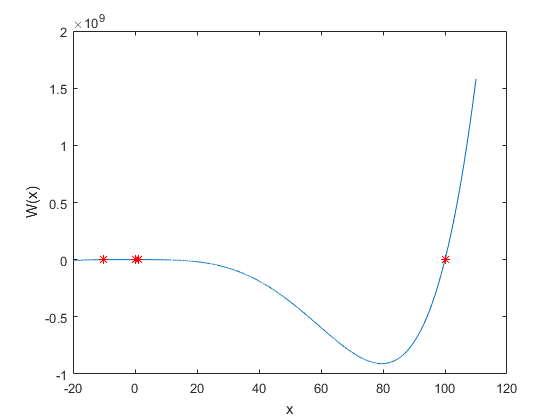
\includegraphics[width=13cm]{obrazDo_Szablonu.png}
	\caption{Wykres funkcji: $w(x)=x^3-91.11x^4-899.989x^3+1100.009x^2-11.091x+1$. Z zaznaczonymi na czerwono wyliczonymi  miejscami zerowymi}
\end{figure}

\section*{IFFALSE}
This we want to keep

\iffalse % ----- START THE CUT ---------

But this part 
$$\int_{-\infty}^\infty\mathrm{d}x\,x^{-2}$$ 
we want to skip

\fi % ---------- END THE CUT -----------

Here it begins again 

\section*{INPUT}
To jest zawartość pliku filename.tex
\subsection{Podsekcja w filename}
Zawartość

\section*{INCLUDEPDF}

\includepdf[pages=3-5]{skr.pdf} % [pages=-] wszystkie

Tekst po skr.pdf
\end{document}